% ##################################################################################################################
\chapter{Quito Metropolitan District}
\label{ch:quito}
\hfill \textbf{Authors:} Rolando Armas, Hernán Aguirre

\editdone{This text has undergone the professional edit. Please no grammatical changes anymore! They are most-probably wrong.}

% ##################################################################################################################
%\gls{dmq}, Ecuador \karen{ What is meant here?  That the city has grown? Or that the whole \gls{dmq}  Ecuador has grown? Please clarify, thanks. I will start a new paragraph}  
%\ah{dmq = Quito Metropolitan District, sorry for the bad reading experience with \gls{...}}

\gls{dmq} (Ecuador) has grown rapidly in recent years, with increasing traffic congestion, gas emissions, pollution and energy use. Our research integrated evolutionary computation, traffic simulation, emission models and data mining tools to gain a better understanding of \gls{dmq}’s complex mobility and transportation system and propose sustainable solutions.

As a first case study \citep[][]{ArmasEtAl_SEAL_2014}, we implemented a mobility scenario to optimize traffic lights under congested conditions. We focused on the
\gls{dmq}’s business district, an area covering 7x3\,square kilometers, as shown in Figure~\ref{fig:quito_fig1}. The area included only the primary and secondary pathways, where free speeds ranged from 30 to 80\,kilometers per hour. The network had approximately 1\,000\,links and was derived from Geofabrik and \gls{osm}. 20\,000 agents were simulated, each with a mobility plan consisting of three main trips: (1) home to work, (2) work to leisure and (3) leisure to home (see Figure~\ref{fig:quito_fig2}). The plans were designed so that all agents moved first from south to north, completely crossing the geographical area of study. In their second trip, the agents moved from north to the central zone of the area under study and in their last trip, from the central zone to the south. Eleven signal lights were located on a main two-way street with flows in south-north and north-south directions (see Figure~\ref{fig:quito_fig1}).

The evolutionary algorithm (the \gls{sop}) together with \gls{matsim} found optimal signal settings of the \gls{dmq} scenario, minimizing average travel time. First, we ran \gls{matsim} for 500\,iterations, to ensure it reached a user equilibrium state without setting any traffic signals. After that, the \gls{sop} evolved a candidate solution population for a number of generations. Each solution represented a configuration of signals (signal control) for the transportation system. At each generation, the \gls{sop} called \gls{matsim} for each candidate solution to evaluate it. \gls{matsim} started from the equilibrium state, setting its signals controls with the tentative solution provided by the \gls{sop} and ran one additional iteration. This iteration's output was used to calculate travel time, which converted and feed back to the \gls{sop} as the fitness value.
%\karen{I don't understand this last sentence. Can we clarify? thanks.} 
%\ah{evolutionary algorithms evaluate their individuals based on a fitness function. Here, a fit individual (i.e., a signal configuration) has a low average travel time. Confusing is that we have two optimizers here, probably interchangeable mentioned. Tried to clarify this with \gls{sop}. }
Figure~\ref{fig:quito_fig2} illustrates the interaction of \gls{matsim} and the \gls{sop}. The first case study \citep[][]{ArmasEtAl_SEAL_2014} provided valuable insights into optimal traffic light setting in the business district of \gls{dmq} under congested conditions. This allowed us to validate problem representation used in the \gls{sop} and effectiveness of the mutation and recombination operators implemented to search solutions. 
%\karen{This whole last paragraph is very ``wordy'' and difficult to understand. Can we simplify and rework?}
%\ah{why?}

Currently, we are scaling up the number of traffic signals to be optimized and testing other mobility scenarios in the same area of study. Our next step is to incorporate an emissions model and use multi-objective evolutionary algorithms \citep[][]{AguireEtAl_EMO_2013} to evolve optimal transportation and mobility system designs of the \gls{dmq}, satisfying multiple criteria for sustainability. These criteria include transportation and mobility policies, accessibility, reduction of emissions, reduction of energy use, as well as social and economic benefit.

\createfigure%
{Study area}%
{Study area}%
{\label{fig:quito_fig1}}%
{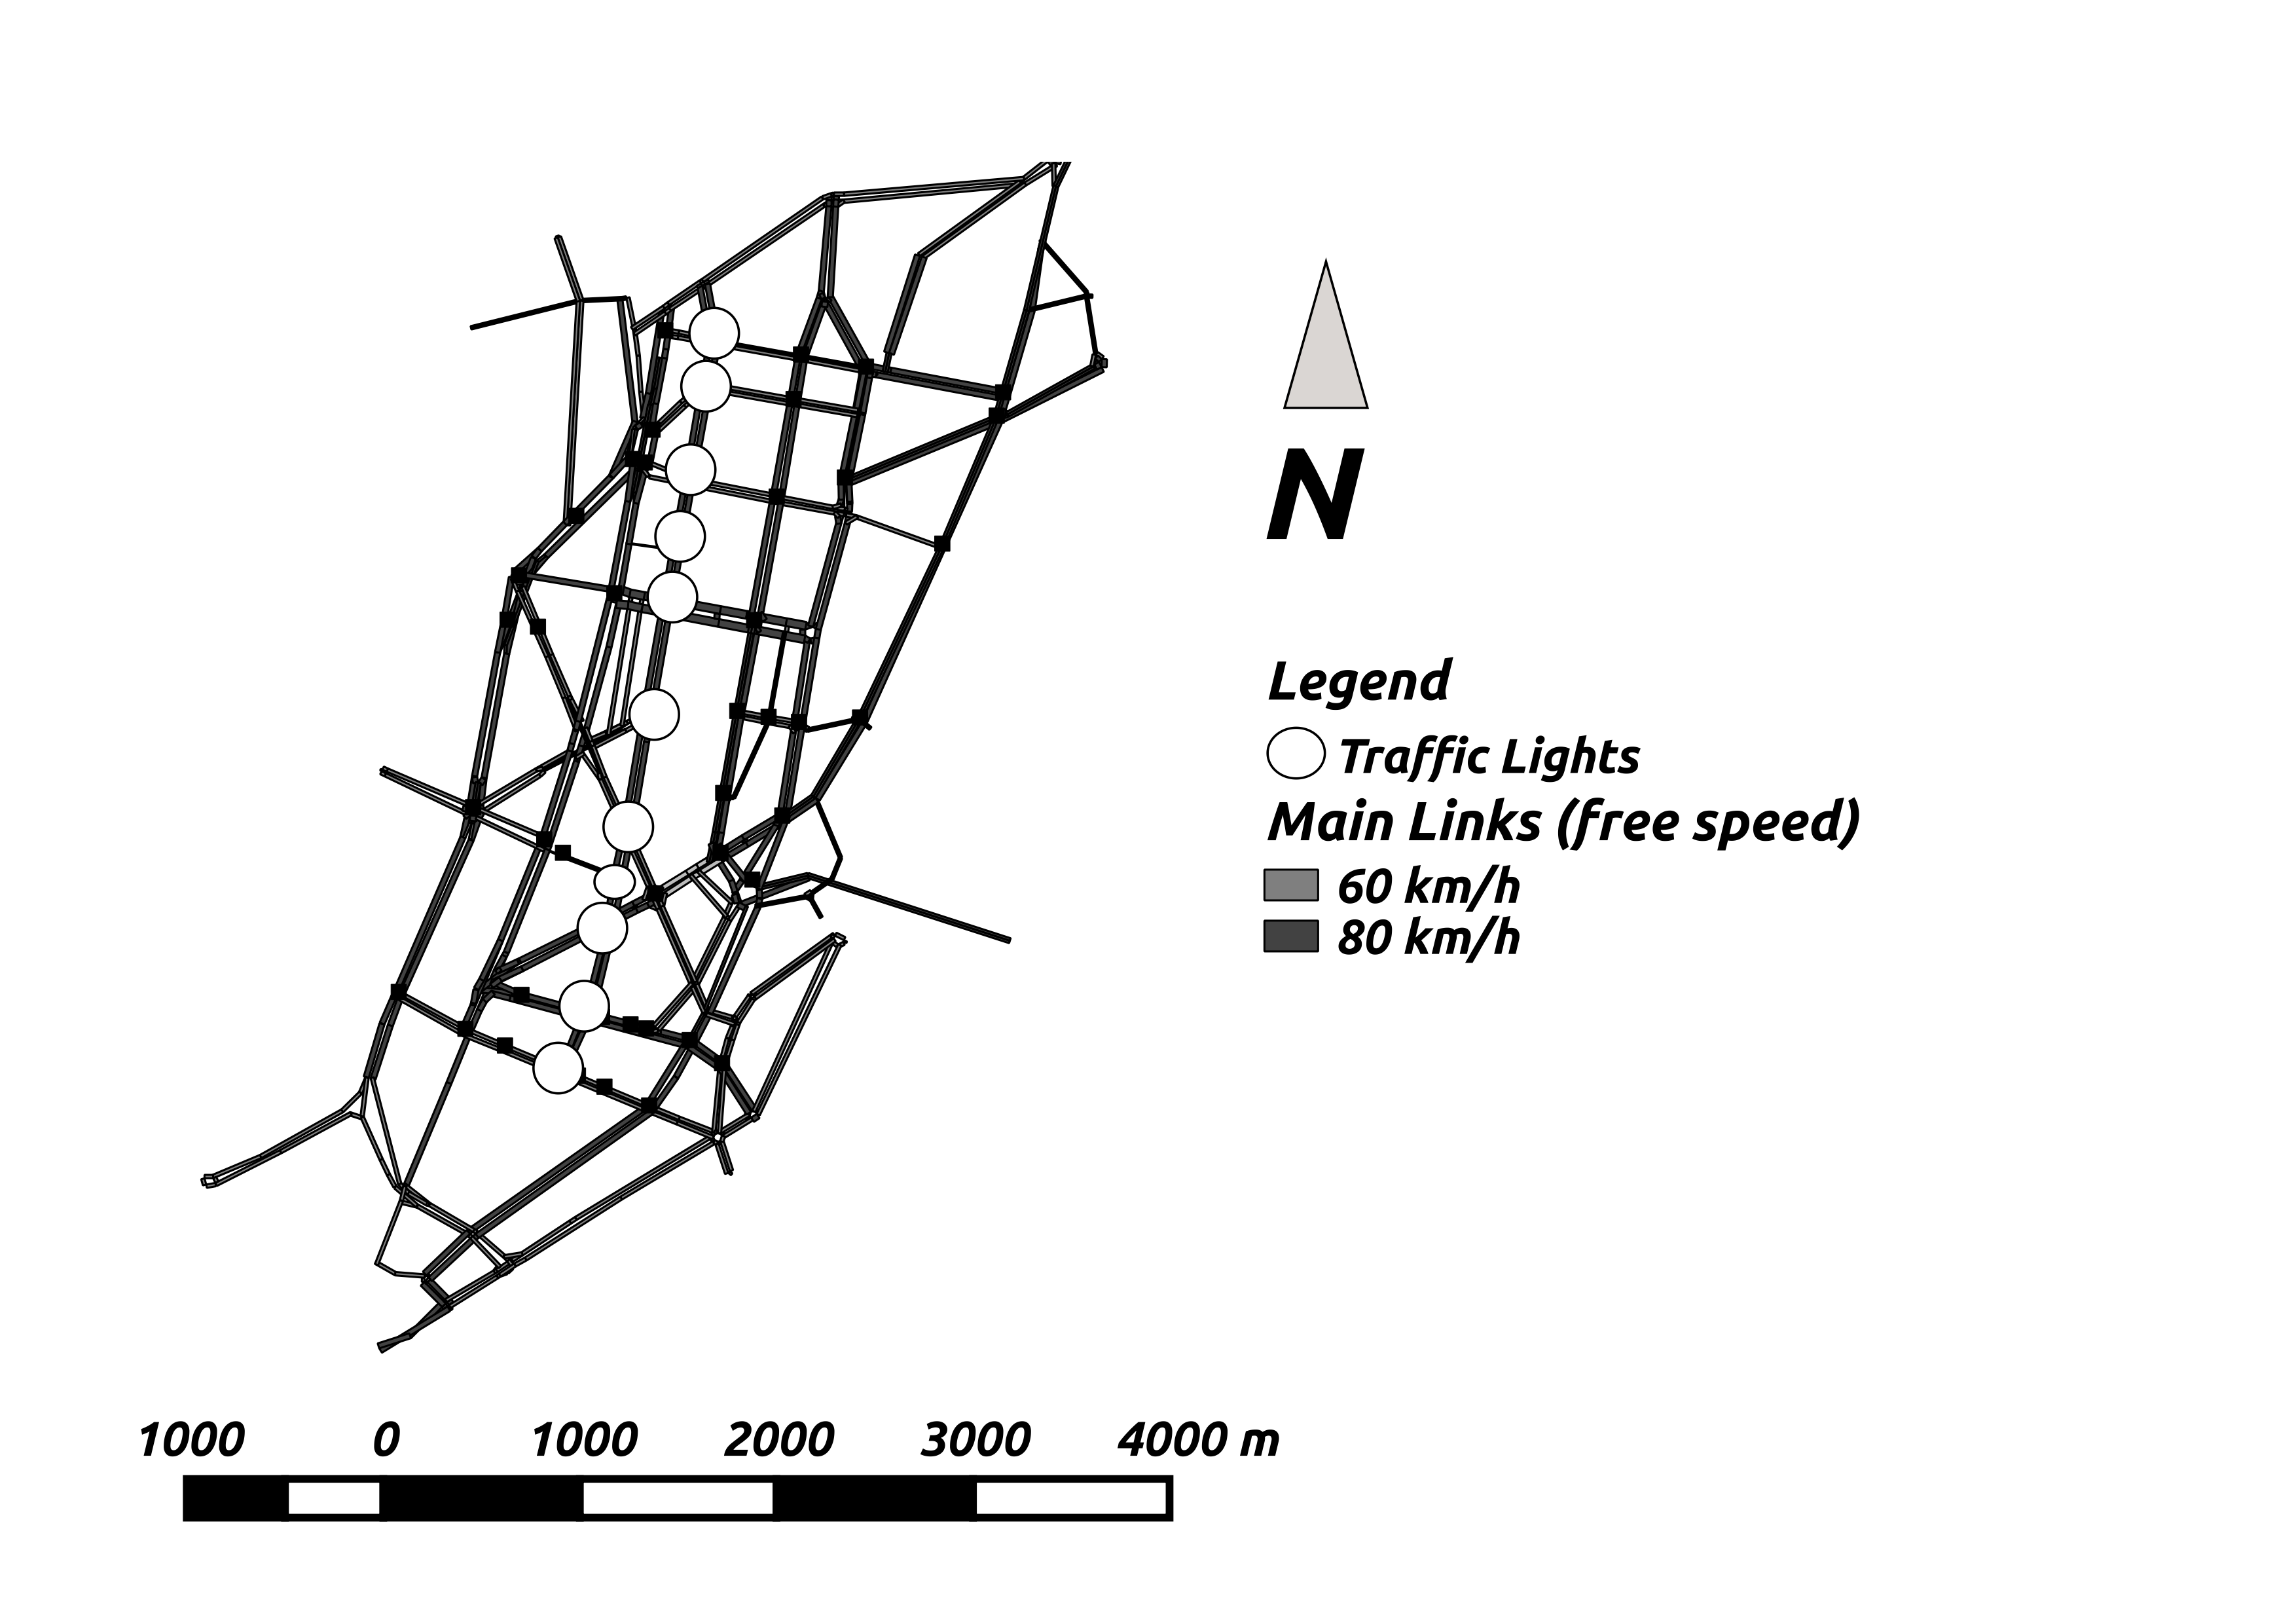
\includegraphics[width=0.7\textwidth, angle=0]{./scenarios/figures/qfig1.png}}%
{}

\createfigure%
{Optimization system}%
{Optimization system}%
{\label{fig:quito_fig2}}%
{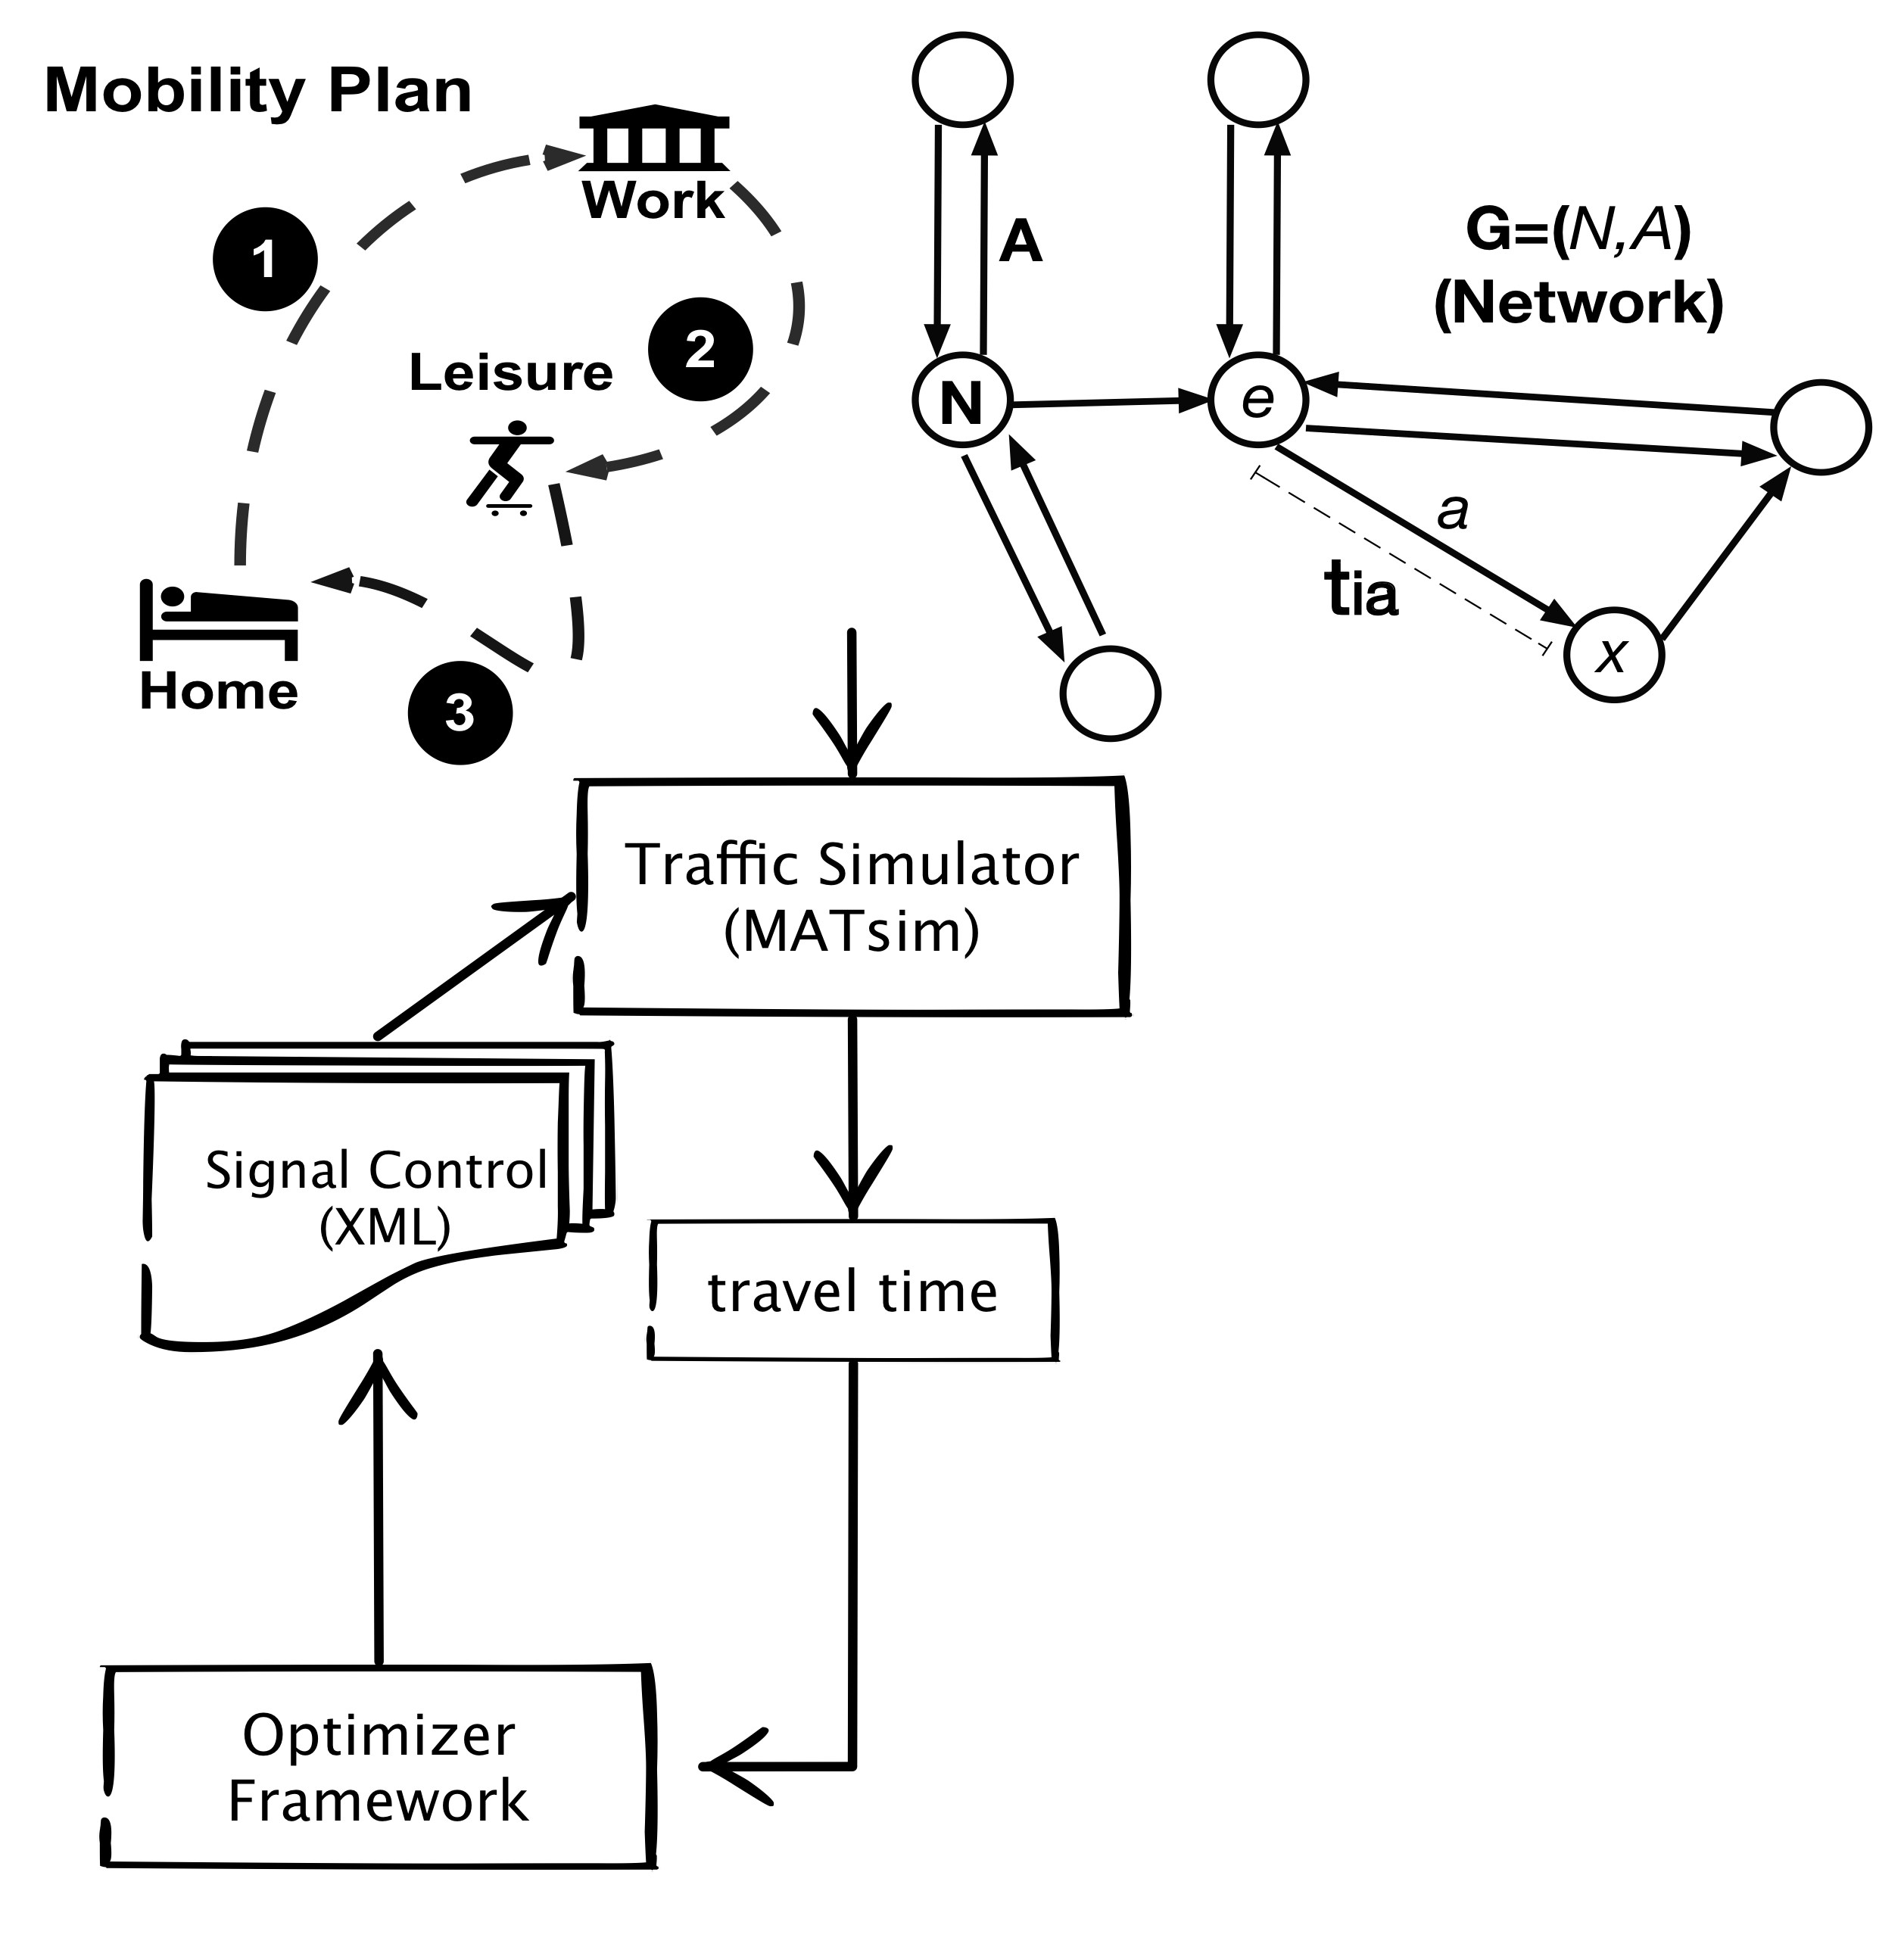
\includegraphics[width=0.7\textwidth, angle=0]{./scenarios/figures/qfig2.png}}%
{}

% ##################################################################################################################


